% !TEX root = ../main.tex

\label{appendix}

\begin{figure}
	\centering
	\begin{subfigure}{.5\textwidth}
		\centering
		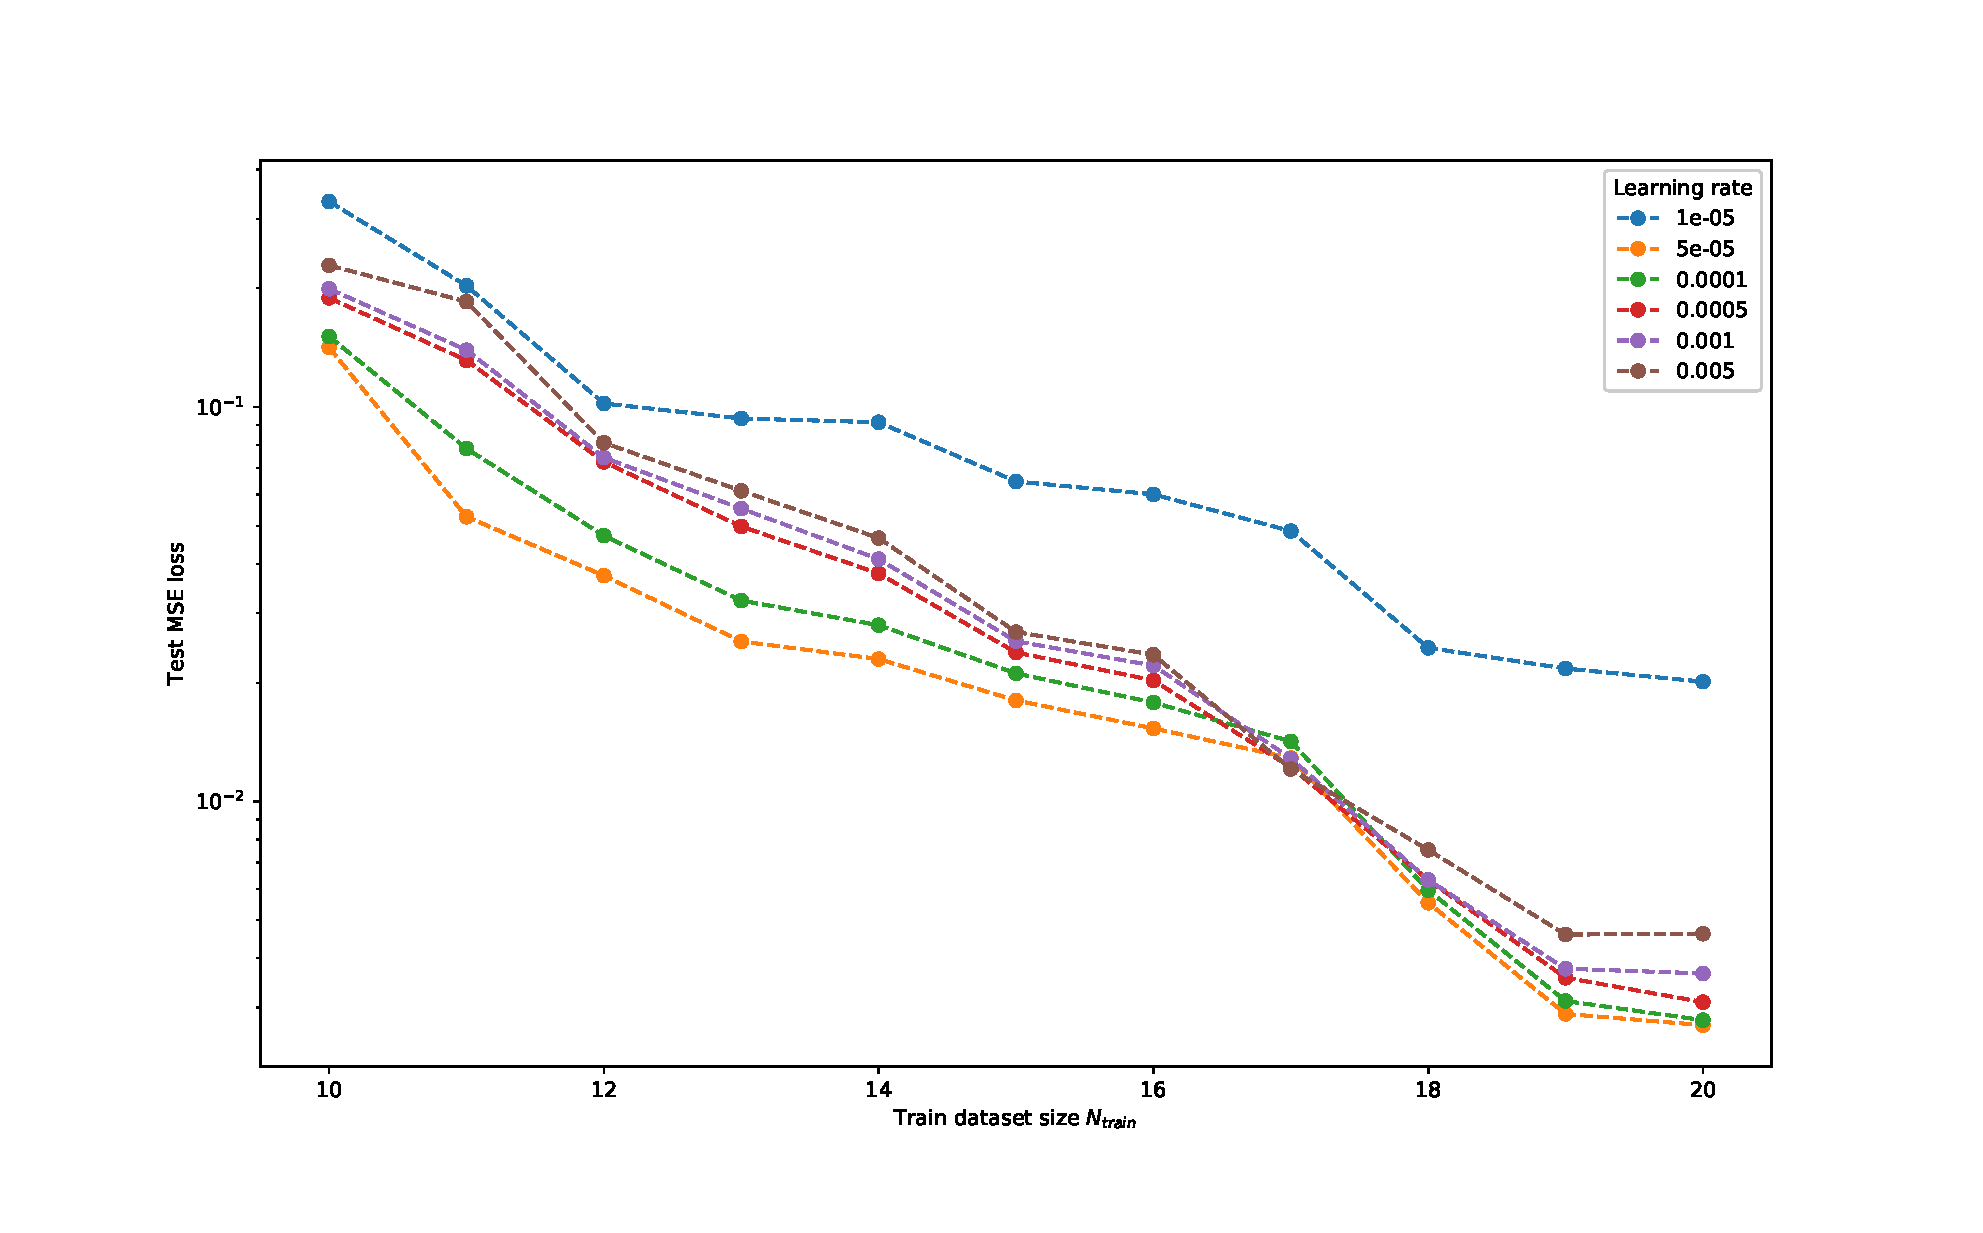
\includegraphics[width=\linewidth]{lr_dim2_m3}
		\caption{2 dimensions}
	\end{subfigure}%
	\begin{subfigure}{.5\textwidth}
		\centering
		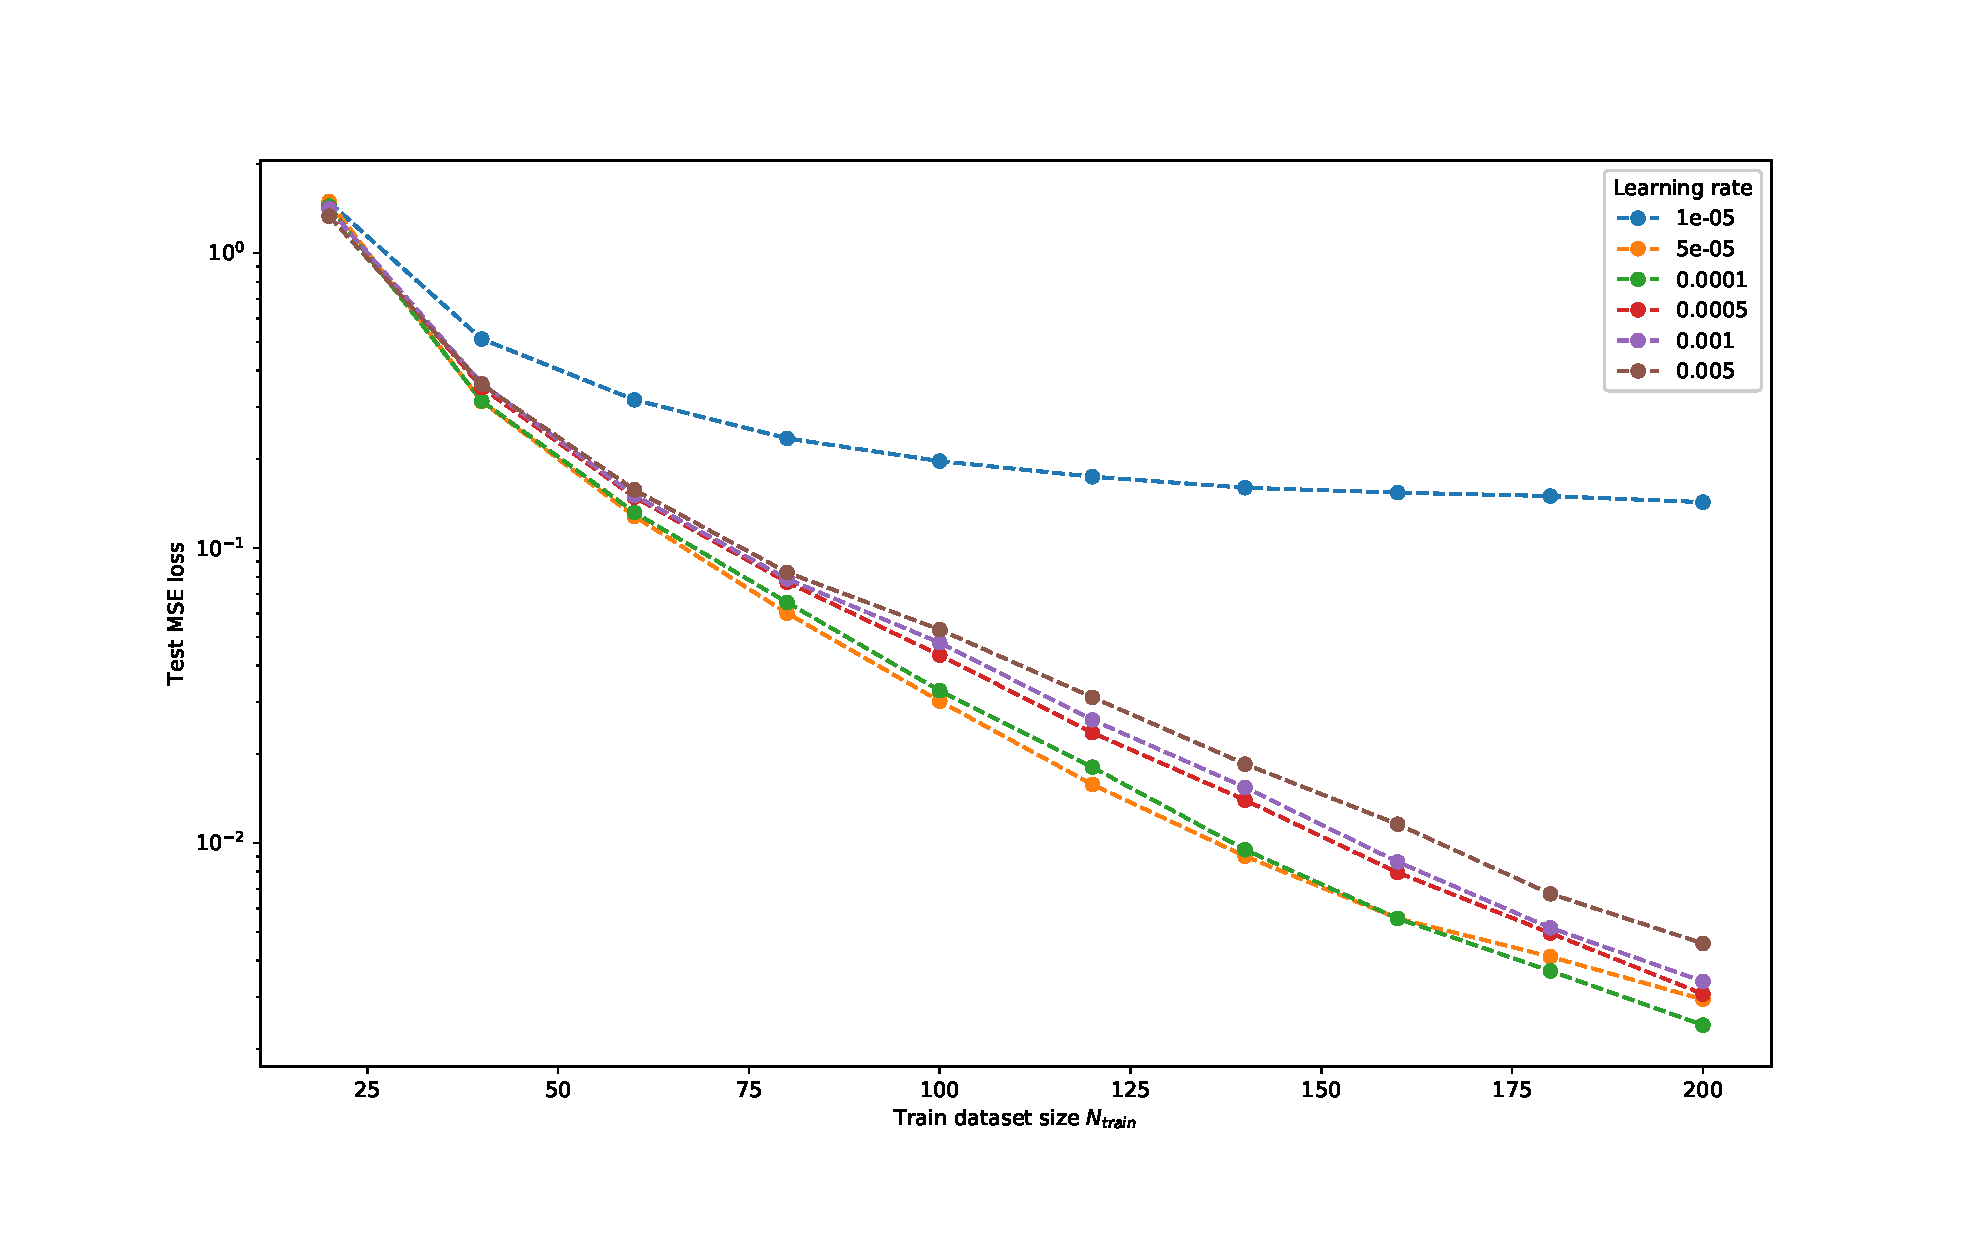
\includegraphics[width=\linewidth]{lr_dim3_m3}
		\caption{3 dimensions}
	\end{subfigure}
	\caption{Comparison of learning rates for Model 3}
	\label{fig:comp_lr_m3}
\end{figure}

\begin{figure}
	\centering
	\begin{subfigure}{.5\textwidth}
		\centering
		\includegraphics[width=\linewidth]{reg_weights}
		\caption{2 dimensions}
	\end{subfigure}%
	\begin{subfigure}{.5\textwidth}
		\centering
		\includegraphics[width=\linewidth]{reg_weights_dim3}
		\caption{3 dimensions}
	\end{subfigure}
	\caption{L2-Regularisation weights on Model 3}
	\label{fig:reg_weights}
\end{figure}


\begin{figure}[ht]
	\centering
	\includegraphics[width=0.7\linewidth]{pnlty_det_large}
	\caption{Different weights $\lambda$ for $L_{DET}$ in 2D}
	\label{fig:pnlty_det_large}
\end{figure}

\begin{figure}[ht]
	\centering
	\includegraphics[width=0.7\linewidth]{pnlty_det_dim3}
	\caption{Different weights $\lambda$ for $L_{DET}$ in 3D}
	\label{fig:pnlty_det_dim3}
\end{figure}

\begin{figure}
	\centering
	\begin{subfigure}{.5\textwidth}
		\centering
		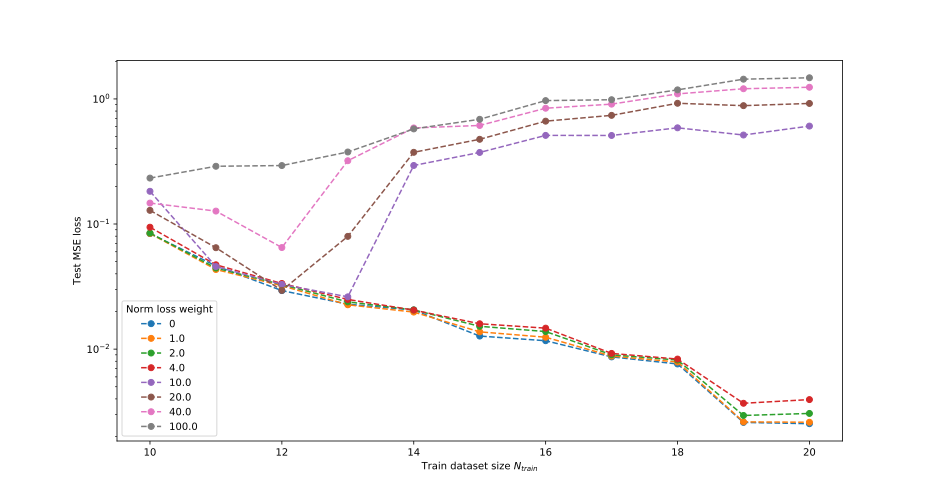
\includegraphics[width=\linewidth]{pnlty_norm}
		\caption{2 dimensions}
	\end{subfigure}%
	\begin{subfigure}{.5\textwidth}
		\centering
		\includegraphics[width=\linewidth]{pnlty_norm_3}
		\caption{3 dimensions}
	\end{subfigure}
	\caption{Penalty Method on the Norm constraint}
	\label{fig:pnlny_norm}
\end{figure}


\begin{figure}[ht]
	\centering
	\includegraphics[width=0.7\linewidth]{normed_det_example}
	\caption{Training for 2 dimensions and $N_{train} = 20$ using the original training and the Physical projection on the determinant with the same training dataset.}
	\label{fig:normed_det_example}
\end{figure}

\begin{figure}
	\centering
	\begin{subfigure}{.5\textwidth}
		\centering
		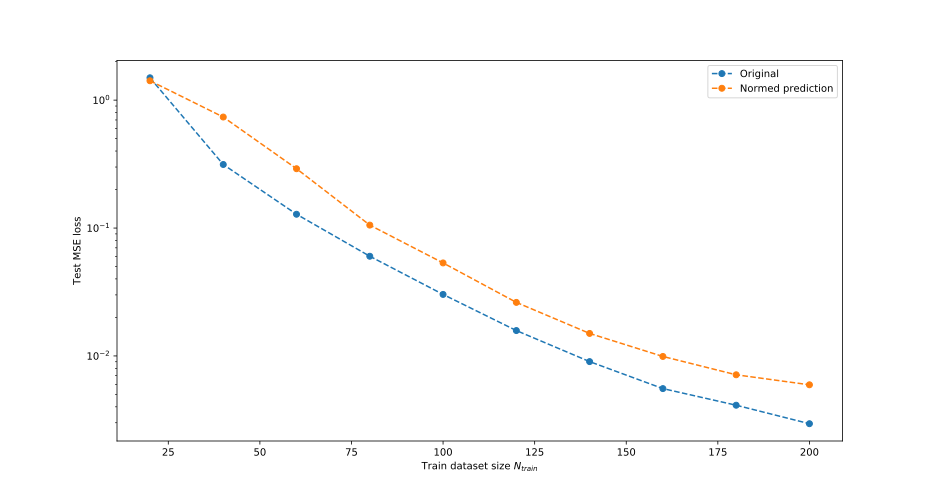
\includegraphics[width=\linewidth]{normed_pred}
		\caption{2 dimensions}
	\end{subfigure}%
	\begin{subfigure}{.5\textwidth}
		\centering
		\includegraphics[width=\linewidth]{normed_pred_3}
		\caption{3 dimensions}
	\end{subfigure}
	\caption{Physical projection on the norm of the prediction}
	\label{fig:normed_pred}
\end{figure}

\begin{figure}[ht]
	\centering
	\includegraphics[width=0.7\linewidth]{normed_pred_example}
	\caption{Analysis of the predictions of a model trained using Physical Projection on the norm compared to the original model. All determinants and norms are scaled such that their mean is equal to one.}
	\label{fig:normed_pred_example}
\end{figure}








\clearpage
